% Options for packages loaded elsewhere
\PassOptionsToPackage{unicode}{hyperref}
\PassOptionsToPackage{hyphens}{url}
\PassOptionsToPackage{dvipsnames,svgnames,x11names}{xcolor}
%
\documentclass[
  10pt,
  dvipsnames,enabledeprecatedfontcommands]{scrartcl}
\usepackage{amsmath,amssymb}
\usepackage{lmodern}
\usepackage{iftex}
\ifPDFTeX
  \usepackage[T1]{fontenc}
  \usepackage[utf8]{inputenc}
  \usepackage{textcomp} % provide euro and other symbols
\else % if luatex or xetex
  \usepackage{unicode-math}
  \defaultfontfeatures{Scale=MatchLowercase}
  \defaultfontfeatures[\rmfamily]{Ligatures=TeX,Scale=1}
\fi
% Use upquote if available, for straight quotes in verbatim environments
\IfFileExists{upquote.sty}{\usepackage{upquote}}{}
\IfFileExists{microtype.sty}{% use microtype if available
  \usepackage[]{microtype}
  \UseMicrotypeSet[protrusion]{basicmath} % disable protrusion for tt fonts
}{}
\usepackage{xcolor}
\usepackage{graphicx}
\makeatletter
\def\maxwidth{\ifdim\Gin@nat@width>\linewidth\linewidth\else\Gin@nat@width\fi}
\def\maxheight{\ifdim\Gin@nat@height>\textheight\textheight\else\Gin@nat@height\fi}
\makeatother
% Scale images if necessary, so that they will not overflow the page
% margins by default, and it is still possible to overwrite the defaults
% using explicit options in \includegraphics[width, height, ...]{}
\setkeys{Gin}{width=\maxwidth,height=\maxheight,keepaspectratio}
% Set default figure placement to htbp
\makeatletter
\def\fps@figure{htbp}
\makeatother
\setlength{\emergencystretch}{3em} % prevent overfull lines
\providecommand{\tightlist}{%
  \setlength{\itemsep}{0pt}\setlength{\parskip}{0pt}}
\setcounter{secnumdepth}{5}
\newlength{\cslhangindent}
\setlength{\cslhangindent}{1.5em}
\newlength{\csllabelwidth}
\setlength{\csllabelwidth}{3em}
\newlength{\cslentryspacingunit} % times entry-spacing
\setlength{\cslentryspacingunit}{\parskip}
\newenvironment{CSLReferences}[2] % #1 hanging-ident, #2 entry spacing
 {% don't indent paragraphs
  \setlength{\parindent}{0pt}
  % turn on hanging indent if param 1 is 1
  \ifodd #1
  \let\oldpar\par
  \def\par{\hangindent=\cslhangindent\oldpar}
  \fi
  % set entry spacing
  \setlength{\parskip}{#2\cslentryspacingunit}
 }%
 {}
\usepackage{calc}
\newcommand{\CSLBlock}[1]{#1\hfill\break}
\newcommand{\CSLLeftMargin}[1]{\parbox[t]{\csllabelwidth}{#1}}
\newcommand{\CSLRightInline}[1]{\parbox[t]{\linewidth - \csllabelwidth}{#1}\break}
\newcommand{\CSLIndent}[1]{\hspace{\cslhangindent}#1}
%\documentclass{article}

% %packages
 \usepackage{booktabs}
\usepackage{subcaption}
\usepackage{multirow}
\usepackage{colortbl}
\usepackage{graphicx}
\usepackage{longtable}
\usepackage{ragged2e}
\usepackage{etex}
%\usepackage{yfonts}
\usepackage{marvosym}
%\usepackage[notextcomp]{kpfonts}
\usepackage[scaled=0.86]{helvet}
\usepackage{nicefrac}
\newcommand*{\QED}{\hfill \footnotesize {\sc Q.e.d.}}
\usepackage{floatrow}
%\usepackage[titletoc]{appendix}
%\renewcommand\thesubsection{\Alph{subsection}}

\usepackage[textsize=footnotesize]{todonotes}
\newcommand{\inbook}[1]{\todo[color=gray!40]{#1}}
\newcommand{\mar}[1]{\todo[color=blue!40]{#1}}
\newcommand{\raf}[1]{\todo[color=olive!40]{#1}}
%\linespread{1.5}
\newcommand{\indep}{\!\perp \!\!\! \perp\!}


\setlength{\parindent}{10pt}
\setlength{\parskip}{1pt}


%language
\usepackage{times}
\usepackage{t1enc}
%\usepackage[utf8x]{inputenc}
%\usepackage[polish]{babel}
%\usepackage{polski}




%AMS
\usepackage{amsfonts}
\usepackage{amssymb}
\usepackage{amsthm}
\usepackage{amsmath}
\usepackage{mathtools}

\usepackage{geometry}
 \geometry{a4paper,left=35mm,top=20mm,}


%environments
\newtheorem{fact}{Fact}



%abbreviations
\newcommand{\ra}{\rangle}
\newcommand{\la}{\langle}
\newcommand{\n}{\neg}
\newcommand{\et}{\wedge}
\newcommand{\jt}{\rightarrow}
\newcommand{\ko}[1]{\forall  #1\,}
\newcommand{\ro}{\leftrightarrow}
\newcommand{\exi}[1]{\exists\, {_{#1}}}
\newcommand{\pr}[1]{\mathsf{P}(#1)}
\newcommand{\cost}{\mathsf{cost}}
\newcommand{\benefit}{\mathsf{benefit}}
\newcommand{\ut}{\mathsf{ut}}

\newcommand{\odds}{\mathsf{Odds}}
\newcommand{\ind}{\mathsf{Ind}}
\newcommand{\nf}[2]{\nicefrac{#1\,}{#2}}
\newcommand{\R}[1]{\texttt{#1}}
\newcommand{\prr}[1]{\mbox{$\mathtt{P}_{prior}(#1)$}}
\newcommand{\prp}[1]{\mbox{$\mathtt{P}_{posterior}(#1)$}}

\newcommand{\s}[1]{\mbox{$\mathsf{#1}$}}


\newtheorem{q}{\color{blue}Question}
\newtheorem{lemma}{Lemma}
\newtheorem{theorem}{Theorem}



%technical intermezzo
%---------------------

\newcommand{\intermezzoa}{
	\begin{minipage}[c]{13cm}
	\begin{center}\rule{10cm}{0.4pt}



	\tiny{\sc Optional Content Starts}
	
	\vspace{-1mm}
	
	\rule{10cm}{0.4pt}\end{center}
	\end{minipage}\nopagebreak 
	}


\newcommand{\intermezzob}{\nopagebreak 
	\begin{minipage}[c]{13cm}
	\begin{center}\rule{10cm}{0.4pt}

	\tiny{\sc Optional Content Ends}
	
	\vspace{-1mm}
	
	\rule{10cm}{0.4pt}\end{center}
	\end{minipage}
	}
%--------------------






















\newtheorem*{reply*}{Reply}
\usepackage{enumitem}
\newcommand{\question}[1]{\begin{enumerate}[resume,leftmargin=0cm,labelsep=0cm,align=left]
\item #1
\end{enumerate}}

\usepackage{float}

% \setbeamertemplate{blocks}[rounded][shadow=true]
% \setbeamertemplate{itemize items}[ball]
% \AtBeginPart{}
% \AtBeginSection{}
% \AtBeginSubsection{}
% \AtBeginSubsubsection{}
% \setlength{\emergencystretch}{0em}
% \setlength{\parskip}{0pt}






\usepackage[authoryear]{natbib}

%\bibliographystyle{apalike}



\usepackage{tikz}
\usetikzlibrary{positioning,shapes,arrows}

\ifLuaTeX
  \usepackage{selnolig}  % disable illegal ligatures
\fi
\IfFileExists{bookmark.sty}{\usepackage{bookmark}}{\usepackage{hyperref}}
\IfFileExists{xurl.sty}{\usepackage{xurl}}{} % add URL line breaks if available
\urlstyle{same} % disable monospaced font for URLs
\hypersetup{
  pdftitle={Second-order Probability, Accuracy and Weight of Evidence},
  pdfauthor={Rafal Urbaniak and Marcello Di Bello},
  colorlinks=true,
  linkcolor={Maroon},
  filecolor={Maroon},
  citecolor={Blue},
  urlcolor={blue},
  pdfcreator={LaTeX via pandoc}}

\title{Second-order Probability, Accuracy and Weight of Evidence}
\author{Rafal Urbaniak and Marcello Di Bello}
\date{November 24, 2022}

\begin{document}
\maketitle

{
\hypersetup{linkcolor=}
\setcounter{tocdepth}{2}
\tableofcontents
}
\vspace{2cm}

\noindent \textbf{DISCLAIMER:}
\textbf{This is a draft of work in progress, please do not cite or distribute without permission.}

\thispagestyle{empty}

\newpage

\begin{quote} \textbf{Abstract.}  \todo{need to write one when done}

\end{quote}

\inbook{this is what a comment about what will go into book looks like; will be globally supressed when generating latex for the journal paper, don't worry about deleting them.}

\hypertarget{introduction}{%
\section{Introduction}\label{introduction}}

A defendant in a criminal case may face multiple items of incriminating
evidence whose strength can at least sometimes be assessed using
probabilities. For example, consider a murder case in which the police
recover trace evidence that matches the defendant. Hair found at the
crime scene matches the defendant's hair (call this evidence
\textsf{hair}). In addition, the defendant owns a dog whose fur matches
the dog fur found in a carpet wrapped around one of the bodies (call
this evidence \textsf{dog}).\footnote{The hair evidence and the dog fur
  evidence are stylized after two items of evidence in the notorious
  1981 Wayne Williams case (Deadman, 1984b, 1984a).} The two matches
suggest that the defendant (and the defendant's dog) must be the source
of the crime traces (call this hypothesis \(\mathsf{source}\)). But how
strong is this evidence, really? What are the fact-finders to make of
it?

The standard story among legal probabilists goes something like this. To
evaluate the strength of the two items of match evidence, we must find
the value of the likelihood ratio:
\[\frac{\pr{\s{dog}\wedge \s{hair} \vert \s{source}}}{\pr{\s{dog}\wedge \s{hair} \vert \neg \s{source}}}\]
For simplicity, the numerator can be equated to one. To fill in the
denominator, an expert provides the relevant random match probabilities.
Suppose the expert testifies that the probability of a random person's
hair matching the reference sample is about 0.0253, and the probability
of a random dog's hair matching the reference sample happens to be about
the same, 0.0256.\footnote{Probabilities have been slightly but not
  unrealistically modified to be closer to each other in order to make a
  conceptual point. The original probabilities were 1/100 for the dog
  fur, and 29/1148 for Wayne Williams' hair. We modified the actual
  reported probabilities slightly to emphasize the point that we will
  elaborate further on: the same first-order probabilities, even when
  they sound precise, may come with different degrees of second-order
  uncertainty.} Presumably, the two matches are independent lines of
evidence. In other words, their random match probabilities must be
independent of each other conditional on the source hypothesis. Then, to
evaluate the overall impact of the evidence on the source hypothesis,
you calculate: \begin{align*}
\pr{\s{dog}\wedge \s{hair} \vert \neg \s{source}} & = \pr{\s{dog} \vert \neg \s{source}} \times \pr{\s{hair} \vert \neg \s{source}} \\
& =  0.0252613 \times  0.025641 = \ensuremath{6.4772626\times 10^{-4}}
\end{align*} This is a very low number. Two such random matches would be
quite a coincidence. Following our advice from Chapter 5, the expert
facilitates your understanding of how this low number should be
interpreted. They show you how the items of match evidence change the
probability of the source hypothesis given a range of possible priors
(Figure \ref{fig:impactOfPoint}). The posterior of .99 is reached as
soon as the prior is higher than 0.061.\footnote{These calculations
  assume that the probability of a match if the suspect and the
  suspect's dog are the sources is one.} While perhaps not sufficient
for outright belief in the source hypothesis, the evidence seems
extremely strong: a minor additional piece of evidence could make the
case against the defendant overwhelming.

\begin{figure}[H]

\begin{center}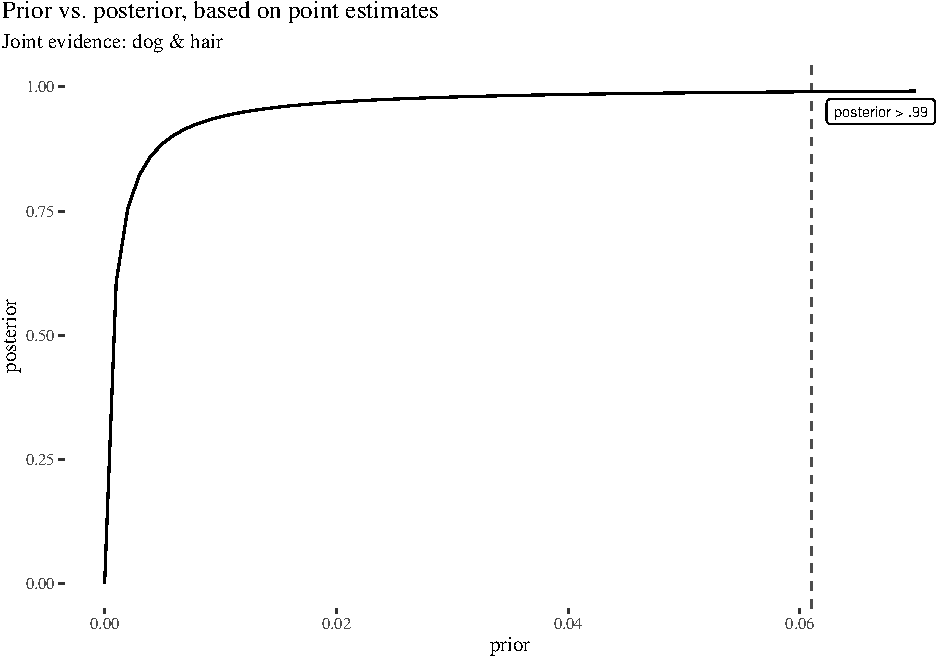
\includegraphics[width=0.6\linewidth]{paper-outline_files/figure-latex/impactOfPoint4-1} \end{center}
\caption{Impact of dog fur and human hair evidence on the prior, point estimates.}
\label{fig:impactOfPoint}
\end{figure}

Unfortunately, this analysis leaves out something crucial. You reflect
on what you have been told and ask the expert: how can you know the
random match probabilities with such precision? Shouldn't we also be
mindful of the uncertainty that may affect these numbers? The expert
agrees, and tells you that in fact the random match probability for the
hair evidence is based on 29 matches found in a database of size 1148,
while the random match probability for the dog evidence is based on
finding two matches in a reference database of size 78.

The expert's answer makes apparent that the precise random match
probabilities do not tell the whole story. Perhaps, the information
about sample sizes is good enough and now you know how to use the
evidence properly.\footnote{This is what, effectively, CITE TARONI seem
  to suggest when they insist the fact-finders should be simply given
  point estimates and information about the study set-up, such as sample
  size. As will transpire, we disagree.} But if you are like most human
beings, you can't. What to do, then?\\
\todo{added this bit to draw attention to this aspect of the Taroni debate, to come back to this}

You ask the expert for guidance: what are reasonable ranges of the
random match probabilities? What are the worst-case and best-case
scenarios? The expert responds with 99\% credible
intervals---specifically, starting with uniform priors, the ranges of
the random match probabilities are (.015,.037) for hair evidence and
(.002, .103) for fur evidence.\footnote{Roughly, the 99\% credible
  interval is the narrowest interval to which the expert thinks the true
  parameter belongs with probability .99. For a discussion of what
  credible intervals are, how they differ from confidence intervals, and
  why confidence intervals should not be used, see Chapter 3.} With this
information, you redo your calculations using the upper bounds of the
two intervals: \(.037\) and \(.103\). The rationale for choosing the
upper bounds is that these numbers result in random match probabilities
that are most favorable to the defendant. Your new calculation yields
the following: \begin{align*}
\mathsf{P}(\s{dog}\wedge \s{hair} \vert \neg \s{source})   & =  .037 \times .103 =.003811.
\end{align*} This number is around 5.88 times greater than the original
estimate. Now the prior probability of the source hypothesis needs to be
higher than 0.274 for the posterior probability to be above .99 (Figure
\ref{fig:impactOfCharitable}). So you are no longer convinced that the
two items of match evidence are strongly incriminating.

\begin{figure}[H]

\begin{center}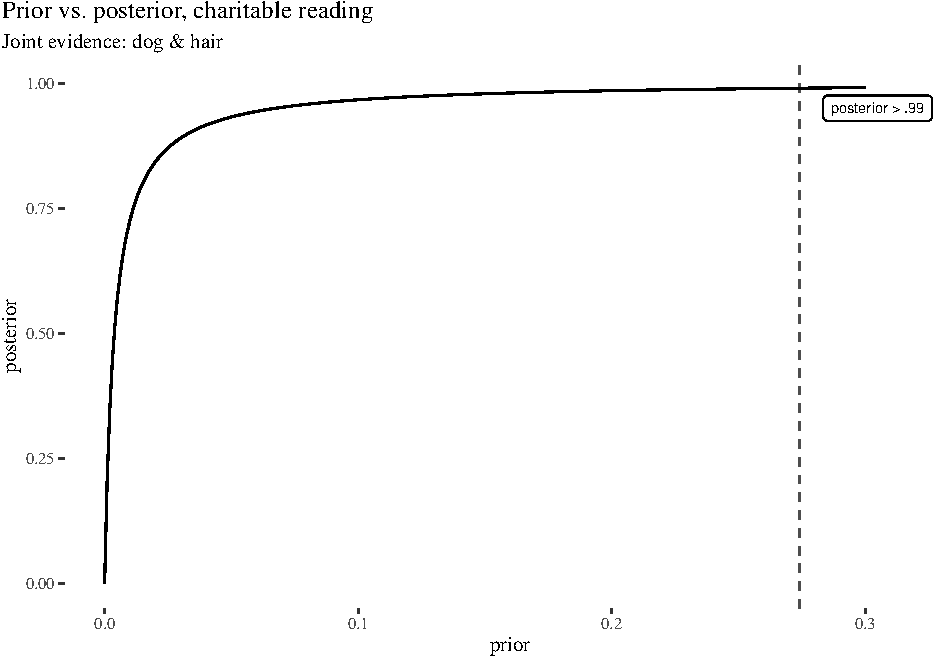
\includegraphics[width=0.6\linewidth]{paper-outline_files/figure-latex/fig:charitableImpact7-1} \end{center}
\caption{Impact of dog fur and human hair evidence on the prior, charitable reading.}
\label{fig:impactOfCharitable}
\end{figure}

This result is puzzling. Are the two items of match evidence strongly
incriminating evidence (as you initially thought) or somewhat weaker (as
the new calculation suggests)? For one thing, using precise random match
probabilities might be too unfavorable toward the defendant. On the
other hand, your new assessment of the evidence based on the upper
bounds might be too \emph{favorable} toward them. Is there a middle way
that avoids overestimating and underestimating the strength of the
evidence?

To see what this middle path looks like, we should reconsider the
calculations you just did. You made an important blunder: you assumed
that because the worst-case probability for one event is \(x\) and the
worst-case probability for another independent event is \(y\), the
worst-case probability for their conjunction is \(xy\). But this
conclusion does not follow if the margin of error (credible interval) is
fixed. The intuitive reason is simple: just because the probability of
an extreme (or larger absolute) value \(x\) for one variable \(X\) is
.01, and so it is for the value \(y\) of another independent variable
\(Y\), it does not follow that the probability that those two
independent variables take values \(x\) and \(y\) simultaneously is the
same. This probability is actually much smaller. The interval
presentation instead of doing us good led us into error.

In general, it is impossible to calculate the credible interval for the
joint distribution based solely on the individual credible intervals
corresponding to the individual events. We need additional information:
the distributions that were used to calculate the intervals for the
probabilities of the individual events. In our example, if you
additionally knew, for instance, that the expert used beta distributions
(as, arguably, they should in this context), you could in principle
calculate the 99\% credible interval for the joint distribution. It
usually will not be the same as whatever the results of multiplication
of individual interval edges, and it is unlikely that a human
fact-finder would be able to correctly run such calculations in their
head even if they knew the functional form of the distributions used.
\footnote{Also, in principle, in more complex contexts, we need further
  information about how the items of evidence are related if we cannot
  take them to be independent.} So providing the fact-finder with
individual intervals, even if further information about the
distributions is provided, might easily mislead.\footnote{Investigation
  of the extent to which the individual interval presentation is
  misleading would be an interesting psychological study.}
\todo{Can you google to see if there is any such study?}

As it turns out, given the reported sample sizes, the 99\% credible
interval for the probability
\(\mathsf{P}(\s{dog}\wedge \s{hair} \vert \neg \s{source})\) is
\((0.000023, 0.002760)\). \todo{the fn was repetitive, compare to fn 5}

The upper bound of this interval would then require the prior
probability of the source hypothesis to be above .215 for the posterior
to be above .99. On this interpretation, the two items of match evidence
are still not quite as strong as you initially thought, but stronger
than what your second calculation indicated.

Still, the interval approach---even the corrected version just
outlined---suffers from a more general problem. Working with intervals
might be useful if the underlying distributions are fairly symmetrical.
But in our case, they might not be. For instance, Figure
\ref{fig:densities} depicts beta densities for dog fur and human hair,
together with sampling-approximated density for the joint evidence. The
distribution for the joint evidence is not symmetric. If you were only
informed about the edges of the interval, you would be oblivious to the
fact that the most likely value (and the bulk of the distribution,
really) does not simply lie in the middle between the edges. Just
because the parameter lies in an interval with some posterior
probability, it does not mean that the ranges near the edges of the
interval are equally likely---the bulk of the density might very well be
closer to one of the edges. Therefore, only relying on the edges can
lead one to either overestimate or underestimate the probabilities at
play. This also means that---following our advice on how to illustrate
the impact of evidence on prior probabilities---a better representation
of the dependence of the posterior on the prior should comprise multiple
possible sampled lines whose density mirrors the density around the
probability of the evidence (Figure \ref{fig:lines}).

\begin{figure}[H]

\begin{center}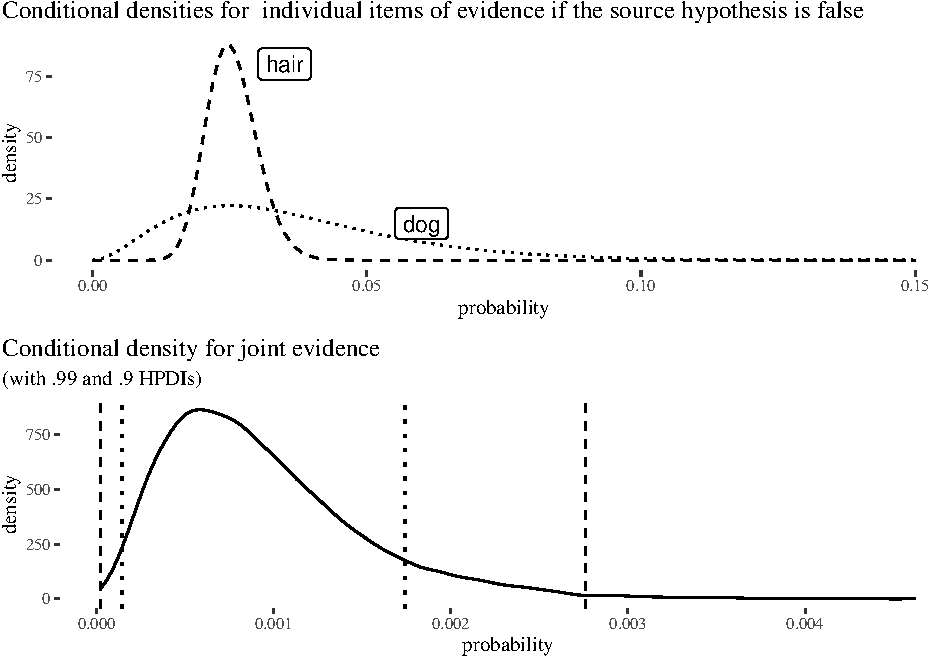
\includegraphics[width=0.8\linewidth]{paper-outline_files/figure-latex/fig:densities-1} \end{center}
\caption{Beta densities for individual items of evidence and the resulting joint density with .99 and .9 highest posterior density intervals, assuming the sample sizes as discussed and independence, with uniform priors.}
\label{fig:densities}
\end{figure}

\begin{figure}[H]

\begin{center}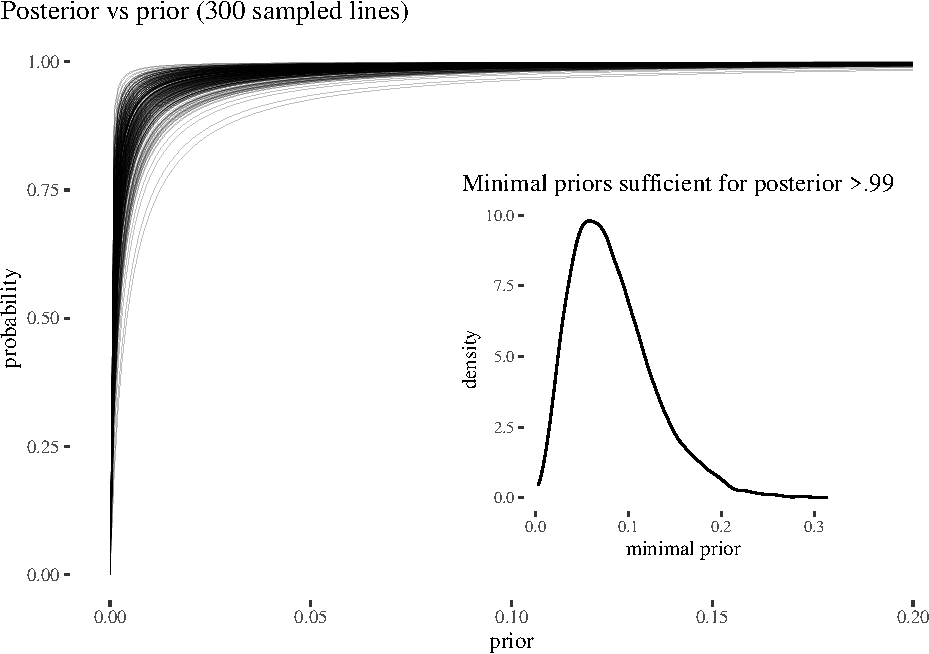
\includegraphics[width=0.6\linewidth]{paper-outline_files/figure-latex/fig:lines5-1} \end{center}

\caption{300 lines illustrating the uncertainty about the dependence of the posterior on the prior given aleatory uncertainty about the evidence, with the distribution of the minimal priors required for the posterior to be above .99.}

\label{fig:lines}

\end{figure}

This, then, is the main claim of this chapter: whenever density
estimates for the probabilities of interest are available (and they
should be available for match evidence and many other items of
scientific evidence if the reliability of a given type of evidence has
been properly studied), those densities should be reported for assessing
the strength of the evidence. This approach avoids hiding actual
aleatory uncertainties under the carpet. It also allows for a balanced
assessment of the evidence, whereas using point estimates or intervals
may exaggerate or underestimate the value of the evidence.

In what follows, we expand on this idea in different directions. Section
\ref{sec:three-probabilism} engages with the philosophical debate about
precise and imprecise probabilism. We argue that both options are
problematic and should be superseded by a higher-order approach to
probability whenever possible. Section \ref{sec:objections} revisits a
recent discussion in the forensic science literature. A prominent view
has it that trial experts, even when they use densities, should present
only first-order probabilities. We disagree and show that reasons of
accuracy maximization sometimes recommend relying on higher-order
probabilities. Section \ref{sec:legal-applications} turns to some legal
applications of higher-order probabilism. We focus on two topics: first,
the role of higher-order probabilities and false positive rates in the
evaluation of DNA evidence; second, how complex bodies of evidence can
be represented by what we call higher-order Bayesian networks.

Before we dive in, one more remark: ost of the time, mathematically, we
do not propose anything radically new---we just put together some of the
items from the standard Bayesian toolkit. The novelty is rather in our
arguing that that these tools are under-appreciated in the legal
scholarship and should be properly used to incorporate second-order
uncertainties in evidence evaluation and incorporation. Perhaps a minor
exception is our explication of the notion of weight, but even here many
related notions are available in information theory, and the novelty
here is not technical, but rather in the argument that they also are
under-appreciated in legal scholarship.
\todo{added this par to preemt Kadane's style pickiness}

\hypertarget{three-probabilisms}{%
\section{Three probabilisms}\label{three-probabilisms}}

\label{sec:three-probabilism}

In introduction we sketched three probabilistic approaches that one
might take for assessing the value of the evidence presented at trial.
The first approach uses precise probabilities; the second uses
intervals; the third uses distributions over probabilities. By relying
on an example featuring two items of match evidence, we suggested that
the third approach is preferable. This section buttresses this claim by
providing principled, philosophical reasons in favor of the third
approach.

The three approaches we considered correspond (roughly) to three ways in
which probabilities can be deployed to model a rational agent's fallible
and evidence-based beliefs about the world. The first approach, known in
the philosophical literature as precise probabilism, posits that an
agent's credal state is modeled by a single, precise probability
measure. The second approach, known as imprecise probabilism, replaces
precise probabilities by sets of probability measures. The third
approach, what we call higher-order probabilism, relies on distributions
over parameter values. There are good reasons to abandon precise
probabilism and endorse higher-order probabilism. Imprecise probabilism
is a step in the right direction, but also suffers from too many
difficulties of its own.

\hypertarget{precise-probabilism}{%
\subsection{Precise probabilism}\label{precise-probabilism}}

Precise probabilism (\textsf{PP}) holds that a rational agent's
uncertainty about a hypothesis is to be represented as a single, precise
probability measure. This is an elegant and simple theory. But
representing our uncertainty about a proposition in terms of a single,
precise probability runs into a number of difficulties. Precise
probabilism fails to capture an important dimension of how our fallible
beliefs reflect the evidence we have (or have not) obtained. A couple of
stylized examples should make the point clear. (For the sake of
simplicity, we will use examples featuring coins, but biases of coins
can be thought of as random match probabilities in the forensic
context.)

\begin{quote}
\textbf{No evidence v. fair coin}
You are about to toss a coin, but have no evidence 
whatsoever about its bias. You are completely ignorant. 
Compare this to the situation in which you know, 
based on overwhelming evidence, that the coin is fair. 
\end{quote}

\noindent On precise probabilism, both scenarios are represented by
assigning a probability of .5 to the outcome \emph{heads}. If you are
completely ignorant, the principle of insufficient evidence suggests
that you assign .5 to both outcomes. Similarly, if you know for sure the
coin is fair, assigning .5 seems the best way to quantify the
uncertainty about the outcome. The agent's evidence in the two scenario
is quite different, but precise probabilities cannot capture this
difference.

\begin{quote}
\textbf{Learning from ignorance}
You toss a coin with unknown bias. You toss it 10 times and observe \emph{heads} 5 times. Suppose you toss it further and observe 50 \emph{heads} in 100 tosses. 
\end{quote}

\noindent Since the coin initially had unknown bias, you should
presumably assign a probability of .5 to both outcomes. After the 10
tosses, you end up again with an estimate of .5. You must have learned
something, but whatever that is, it is not modeled by precise
probabilities. When you toss the coin 100 times and observe 50 heads,
you learn something. But your precise probability assessment will again
be .5.

These examples suggest that precise probabilism is not appropriately
responsive to evidence. It ends up assigning the same probability in
situations in which one's evidence is quite different: when no evidence
is available about the coin's bias; when there is little evidence that
the coin is fair (say, after only 10 tosses); and when there is strong
evidence that the coin is fair (say, after 100 tosses). The general
problem is, precise probability captures the value around which your
uncertainty should be centered, but fails to capture how centered it
should be given the evidence.\footnote{Precise probabilism suffers from
  other difficulties. For example, it has problems with formulating a
  sensible method of probabilistic opinion aggregation Stewart \&
  Quintana (2018). A seemingly intuitive constraint is that if every
  member agrees that \(X\) and \(Y\) are probabilistically independent,
  the aggregated credence should respect this. But this is hard to
  achieve if we stick to \s{PP} (Dietrich \& List, 2016). For instance,
  a \emph{prima facie} obvious method of linear pooling does not respect
  this. Consider probabilistic measures \(p\) and \(q\) such that
  \(p(X) = p(Y) = p(X\vert Y) = 1/3\) and
  \(q(X) = q(Y) = q(X\vert Y) = 2/3\). On both measures, taken
  separately, \(X\) and \(Y\) are independent. Now take the average,
  \(r=p/2+q/2\). Then \(r(X\cap Y) = 5/18 \neq r(X)r(Y)=1/4\).}

\hypertarget{imprecise-probabilism}{%
\subsection{Imprecise probabilism}\label{imprecise-probabilism}}

What if we give up the assumption that probability assignments should be
precise? Imprecise probabilism (\textsf{IP}) holds that an agent's
credal stance towards a hypothesis is to be represented by means of a
\emph{set of probability measures}, typically called a representor
\(\mathbb{P}\), rather than a single measure \(\mathsf{P}\). The
representor should include all and only those probability measures which
are compatible with the evidence. For instance, if an agent knows that
the coin is fair, their credal state would be represented by the
singleton set \(\{\mathsf{P}\}\), where \(\mathsf{P}\) is a probability
measure which assigns \(.5\) to \emph{heads}. If, on the other hand, the
agent knows nothing about the coin's bias, their credal state would be
represented by the set of all probabilistic measures, since none of them
is excluded by the available evidence. Note that the set of probability
measures does not represent admissible options that the agent could
legitimately pick from. Rather, the agent's credal state is essentially
imprecise and should be represented by means of the entire set of
probability measures.\footnote{For the development of imprecise
  probabilism, see Keynes (1921); Levi (1974); Gärdenfors \& Sahlin
  (1982); Kaplan (1968); Joyce (2005); Fraassen (2006); Sturgeon (2008);
  Walley (1991). S. Bradley (2019) is a good source of further
  references. Imprecise probabilism shares some similarities with what
  we might call \textbf{interval probabilism} (Kyburg, 1961; Kyburg Jr
  \& Teng, 2001). On interval probabilism, precise probabilities are
  replaced by intervals of probabilities. On imprecise probabilism,
  instead, precise probabilities are replaced by sets of probabilities.
  This makes imprecise probabilism more general, since the probabilities
  of a proposition in the representor set do not have to form a closed
  interval. As we have already noted, intervals do not contain
  probabilistic information sufficient to guide reasoning with multiple
  items of evidence. So we focus on \s{IP}, which is the more promising
  approach.}

Imprecise probabilism, at least \emph{prima facie}, offers a
straightforward picture of learning from evidence, that is a natural
extension of the classical Bayesian approach. When faced with new
evidence \(E\) between time \(t_0\) and \(t_1\), the representor set
should be updated point-wise, running the standard Bayesian updating on
each probability measure in the representor:
\begin{align*} \label{eq:updateRepresentor}
\mathbb{P}_{t_1} = \{\mathsf{P}_{t_1}\vert \exists\, {\mathsf{P}_{t_0} \!\in  \mathbb{P}_{t_0}}\,\, \forall\, {H}\,\, \left[\mathsf{P}_{t_1}(H)=\mathsf{P}_{t_0}(H \vert E)\right] \}.
\end{align*}

\noindent The hope is that, if we start with a range of probabilities
that is not extremely wide, point-wise learning will behave
appropriately. For instance, if we start with a prior probability of
\emph{heads} equal to .4 or .6, then those measure should be updated to
something closer to \(.5\) once we learn that a given coin has already
been tossed ten times with the observed number of heads equal 5 (call
this evidence \(E\)). This would mean that if the initial range of
values was \([.4,.6]\) the posterior range of values should be more
narrow. But even this seemingly straightforward piece of reasoning is
hard to model without using densities. For to calculate
\(\pr{\s{heads}\vert E}\) we need to calculate
\(\pr{E \vert \s{heads}}\pr{\s{heads}}\) and divide it by
\(\pr{E} = \pr{E \vert \s{heads}}\pr{\s{heads}} + \pr{E} = \pr{E \vert \neg \s{heads}}\pr{\neg \s{heads}}\).
The tricky part is obtaining the conditional probabilities
\(\pr{E \vert \s{heads}}\) and \(\pr{E \vert \neg \s{heads}}\) in a
principled manner without explicitly going second-order, estimating the
parameter value and using beta distributions.

The situation is even more difficult if we start with complete lack of
knowledge, as imprecise probabilism runs into the problem of
\textbf{belief inertia} (Levi, 1980). Say you start tossing a coin
knowing nothing about its bias. The range of possibilities is \([0,1]\).
After a few tosses, if you observed at least one tail and one heads, you
can exclude the measures assigning 0 or 1 to \emph{heads}. But what else
have you learned? If you are to update your representor set point-wise,
you will end up with the same representor set. Consequently, the edges
of your resulting interval will remain the same. In the end, it is not
clear how you are supposed to learn anything if you start from complete
ignorance.\footnote{Here's another example from Rinard (2013). Either
  all the marbles in the urn are green (\(H_1\)), or exactly one tenth
  of the marbles are green (\(H_2\)). Your initial credence \([0,1]\) in
  each. Then you learn that a marble drawn at random from the urn is
  green (\(E\)). After conditionalizing each function in your
  representor on this evidence, you end up with the the same spread of
  values for \(H_1\) that you had before learning \(E\), and no matter
  how many marbles are sampled from the urn and found to be green.}

Some downplay the problem of belief inertia. They insist that vacuous
priors should not be used and that imprecise probabilism gives the right
results when the priors are non-vacuous. After all, if you started with
knowing truly nothing, then perhaps it is right to conclude that you
will never learn anything. Another strategy is to say that, in a state
of complete ignorance, a special updating rule should be
deployed.\footnote{Elkin (2017) suggests the rule of
  \emph{credal set replacement} that recommends that upon receiving
  evidence the agent should drop measures rendered implausible, and add
  all non-extreme plausible probability measures. This, however, is
  tricky. One needs a separate account of what makes a distribution
  plausible or not, as well as a principled account of why one should
  use a separate special update rule when starting with complete
  ignorance.} But no matter what we think about belief inertia, other
problems plague imprecise probabilism. Two more problems are
particularly pressing.

One problem is that imprecise probabilism fails to capture intuitions we
have about evidence and uncertainty in a number of scenarios. Consider
this example:

\begin{quote}
\textbf{Even v. uneven bias:}
 You have two coins and you know, for sure, that the probability of getting heads is .4, if you toss one coin, and .6, if you toss the other coin. But you do not know which is which. You pick one of the two at random and toss it.  Contrast this with an uneven case. You have four coins and you know that three of them have bias $.4$ and one of them has bias $.6$. You pick a coin at random and plan to toss it. You should be three times more confident that the probability of getting heads is .4. rather than .6.
\end{quote}

\noindent The first situation can be easily represented by imprecise
probabilism. The representor would contain two probability measures, one
that assigns .4. and the other that assigns .6 to the hypothesis `this
coin lands heads'. But imprecise probabilism cannot represent the second
situation, at least not without moving to higher-order probabilities or
assigning probabilities to chance hypotheses, in which case it is no
longer clear whether the object-level imprecision performs any valuable
task.\footnote{Other scenarios can be constructed in which imprecise
  probabilism fails to capture distinctive intuitions about evidence and
  uncertainty; see, for example, (Rinard, 2013). Suppose you know of two
  urns, \textsf{GREEN} and \textsf{MYSTERY}. You are certain
  \textsf{GREEN} contains only green marbles, but have no information
  about \textsf{MYSTERY}. A marble will be drawn at random from each.
  You should be certain that the marble drawn from \textsf{GREEN} will
  be green (\(G\)), and you should be more confident about this than
  about the proposition that the marble from \textsf{MYSTERY} will be
  green (\(M\)). In line with how lack of information is to be
  represented on \textsf{IP}, for each \(r\in [0,1]\) your representor
  contains a \(\mathsf{P}\) with \(\pr{M}=r\). But then, it also
  contains one with \(\pr{M}=1\). This means that it is not the case
  that for any probability measure \(\mathsf{P}\) in your representor,
  \(\mathsf{P}(G) > \mathsf{P}(M)\), that is, it is not the case that RA
  is more confident of \(G\) than of \(M\). This is highly
  counter-intuitive.}

Second, besides descriptive inadequacy, an even deeper, foundational
problem exists for imprecise probabilism. This problem arises when we
attempt to measure the accuracy of a representor set of probability
measures. Workable \emph{scoring rules} exists for measuring the
accuracy of a single, precise credence function, such as the Brier
score. These rules measure the distance between one's credence function
(or probability measure) and the actual value. A requirement of scoring
rules is that they be \emph{proper}: any agent will score their own
credence function to be more accurate than every other credence
function. After all, if an agent thought a different credence was more
accurate, they should switch to it. Proper scoring rules are then used
to formulate accuracy-based arguments for precise probabilism. These
arguments show (roughly) that, if your precise credence follows the
axioms of probability theory, no other credence is going to be more
accurate than yours whatever the facts are. Can the same be done for
imprecise probabilism? It seems not. Impossibility theorems demonstrate
that no proper scoring rules are available for representor sets. So, as
many have noted, the prospects for an accuracy-based argument for
imprecise probabilism look dim (Campbell-Moore, 2020; Mayo-Wilson \&
Wheeler, 2016; Schoenfield, 2017; Seidenfeld, Schervish, \& Kadane,
2012). Moreover, as shown by Schoenfield (2017), if an accuracy measure
satisfies certain plausible formal constraints, it will never strictly
recommend an imprecise stance, as for any imprecise stance there will be
a precise one with at least the same accuracy.

\hypertarget{higher-order-probabilism}{%
\subsection{Higher-order probabilism}\label{higher-order-probabilism}}

There is, however, a view in the neighborhood that fares better: a
second-order perspective. In fact, some of the comments by the
proponents of imprecise probabilism tend to go in this direction. For
instance, Seamus Bradley compares the measures in a representor to
committee members, each voting on a particular issue, say the true bias
of a coin. As they acquire more evidence, the committee members will
often converge on a specific chance hypothesis. He writes (S. Bradley,
2012, p. 157):

\begin{quote}
\dots the committee members are ''bunching up''. Whatever measure you put over the set of probability functions---whatever ''second order probability'' you use---the ''mass'' of this measure gets more and more concentrated around the true chance hypothesis'.
\end{quote}

\noindent Note, however, that such bunching up cannot be modeled by
imprecise probabilism. Joyce (2005), in a paper defending imprecise
probabilism, in fact uses a density over chance hypotheses to account
for the notion of evidential weight. The idea that one should use
higher-order probabilities has also been suggested by critics of
imprecise probabilism. For example, Carr (2020) argues that sometimes
evidence requires uncertainty about what credences to have. Carr,
however, does not articulate this suggestion more fully, does not
develop it formally, and does not explain how her approach would fare
against the difficulties affecting precise ad imprecise probabilism.

The key idea of the higher-order approach we propose is that uncertainty
is not a single-dimensional thing to be mapped on a single
one-dimensional scale such as a real line. It is the whole shape of the
whole distribution over parameter values that should be taken under
consideration.\footnote{Bradley admits this much (S. Bradley, 2012, p.
  90), and so does Konek (Konek, 2013, p. 59). For instance, Konek
  disagrees with: (1) \(X\) is more probable than \(Y\) just in case
  \(p(X)>p(Y)\), (2) \(D\) positively supports \(H\) if
  \(p_D(H)> p(H)\), or (3) \(A\) is preferable to \(B\) just in case the
  expected utility of \(A\) w.r.t. \(p\) is larger than that of \(B\).}
From this perspective, when an agent is asked about their credal stance
towards \(X\), they can refuse to summarize it in terms of a point value
\(\mathsf{P}(X)\). They can instead express their credal stance in terms
of a probability (density) distribution \(f_x\) treating
\(\mathsf{P}(X)\) as a random variable. To be sure, an agent's credal
state toward \(X\) could sometimes be usefully represented by the
expectation\\
\[\int_{0}^{1} x f(x) \, dx\] as the precise, object-level credence in
\(X\), where \(f\) is the probability density over possible object-level
probability values. But this need not always be the case. If the
probability density \(f\) is not sufficiently concentrated around a
single value, a one-point summary might fail to do justice to the
nuances of the agent's credal state.\footnote{This approach lines up
  with common practice in Bayesian statistics, where the primary role of
  uncertainty representation is assigned to the whole distribution.
  Summaries such as the mean, mode standard deviation, mean absolute
  deviation, or highest posterior density intervals are only succinct
  ways for representing the uncertainty of a given scenario. Whether the
  expectation should be used in betting behavior is a separate problem.
  Here we focus on epistemic issues.} For example, consider again the
scenario in which the agent knows that the bias of the coin is either .4
or .6 but the former is three times more likely. Representing the
agent's credal state with the expectation
\(\mathsf{P}(X) = .75 \times .4 + .25 \times .6 = .45\) would be
inadequate as it would fail to capture the agent's belief that the two
biases are uneven.

The higher-order approach can easily model all the challenging scenarios
we discussed so far in the manner illustrated in Figure
\ref{fig:evidenceResponse}. In particular, the scenario in which the two
biases of the coin are not equally likely---which imprecise probabilism
cannot model---can be easily modeled within high-order probabilism by
assigning different probabilities to the two biases.

\begin{figure}[t]

\begin{center}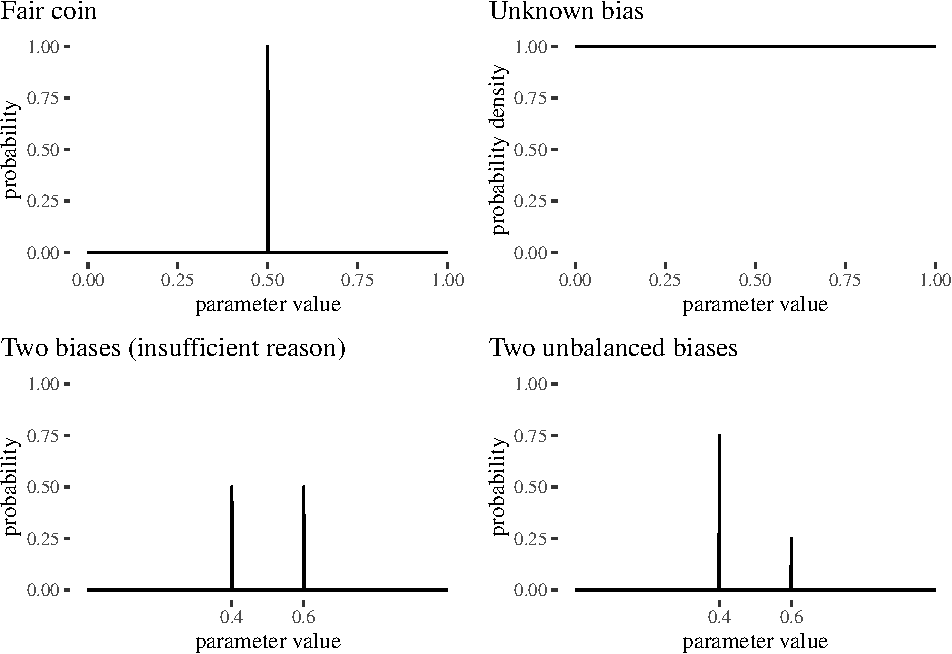
\includegraphics[width=0.8\linewidth]{paper-outline_files/figure-latex/fig:evidenceResponse2-1} \end{center}
\caption{Examples of higher-order distributions for scenarios brought up in the literature.}
\label{fig:evidenceResponse}
\end{figure}

Besides its flexibility in modelling uncertainty, higher-order
probabilism does not fall prey to belief inertia. Consider a situation
in which you have no idea about the bias of a coin. So you start with a
uniform density over \([0,1]\) as your prior. By using binomial
probabilities as likelihoods, observing any non-zero number of heads
will exclude 0 and observing any non-zero number of tails will exclude 1
from the basis of the posterior. The posterior distribution will become
more centered around the parameter estimate as the observations come in.
Figure \ref{fig:intertia2} shows---starting with a uniform prior
distribution--- how the posterior distribution changes after successive
observations of heads, heads again, and then tails.\footnote{More
  generally, learning about frequencies, assuming independence and
  constant probability for all the observations, is modeled the Bayes
  way. You start with some prior density \(p\) over the parameter
  values. If you start with complete lack of information, \(p\) should
  be uniform. Then, you observe the data \(D\) which is the number of
  successes \(s\) in a certain number of observations \(n\). For each
  particular possible value \(\theta\) of the parameter, the probability
  of \(D\) conditional on \(\theta\) follows the binomial distribution.
  The probability of \(D\) is obtained by integration. That is:
  \begin{align*}
  p(\theta \vert D) & = \frac{p(D\vert \theta)p(\theta)}{p(D)}\\
  & = \frac{\theta^s (1-\theta)^{(n - s)}p(\theta)}{\int (\theta')^s (1-\theta')^{(n - s)}p(\theta')\,\, d\theta'}.
  \end{align*}}

\begin{figure}[t]

\begin{center}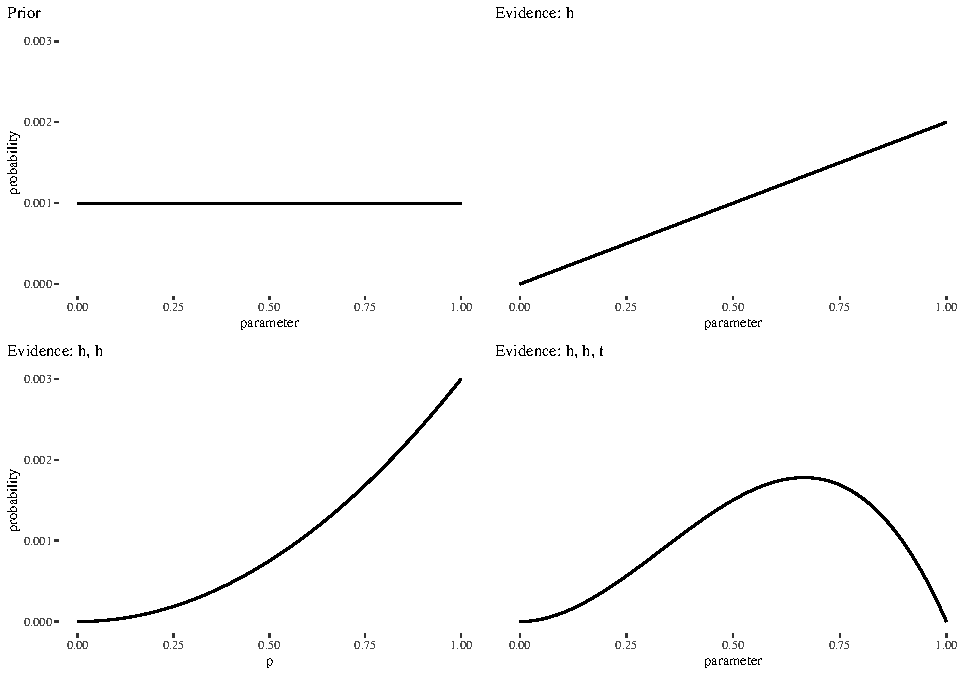
\includegraphics[width=0.8\linewidth]{paper-outline_files/figure-latex/fig:inertia3-1} \end{center}
\caption{As observations of heads, heads and tails come in, extreme parameter values drop out of the picture and the posterior is shaped by the evidence.}
\label{fig:intertia2}
\end{figure}

A further advantage of high-order probabilism over imprecise probabilism
is that the prospects for accuracy-based arguments are not foreclosed.
This is a significant shortcoming of imprecise probabilism, especially
because such arguments exist for precise probabilism. One can show that
there exist proper scoring rules for higher-order probabilism. These
rules can then be used to formulate accuracy-based arguments. Another
interesting feature of the framework is that the point made by
Schoenfield against imprecise probabilism does not apply: there are
cases in which accuracy considerations recommend an imprecise stance
(that is, a multi-modal distribution) over a precise one (Urbaniak, 2022
manuscript).

All in all, higher-order probabilism outperforms both precise and
imprecise probabilism, at the descriptive as well as the normative
level. From a descriptive standpoint, higher-order probabilism can
easily model a variety of scenarios that cannot be adequately modeled by
the other versions of probabilism. From a normative standpoint, accuracy
maximization may sometimes recommend that a rational agent represent
their credal state with a distribution over probability values rather
than a precise probability measure (more on this in the next section).

\hypertarget{objections}{%
\section{Objections}\label{objections}}

\label{sec:objections}

This section addresses a number of conceptual difficulties that may
arise in using higher-order probabilities, with focus on those brought
up by prominent legal evidence scholars. In discussing these conceptual
issues, we will formulate an accuracy-based argument that higher-order
probabilities are preferable to precise probabilities.

\hypertarget{the-taroni-sjerps-debate}{%
\subsection{The Taroni-Sjerps debate}\label{the-taroni-sjerps-debate}}

Our treatment will be centered around a discussion initiated by Taroni,
Bozza, Biedermann, \& Aitken (2015), who argue extensively that trial
experts should avoid report higher-order densities, and should only
report point estimates. Their point of departure is a reflection on
match evidence.

Say an expert reports at trial that the sample from the crime scene
matches the defendant. The significance of this match should be
evaluated in light of the population frequency \(\theta\) of the
matching profile. This frequency, however, cannot be known for sure and
must instead be estimated.

The expert will estimate the true parameter \(\theta\) by means of a
probability distribution \(p(\theta)\) over its possible values. For
example, if the observations are realizations of independent and
identically distributed Bernoulli trails given \(\theta\), the expert's
uncertainty about \(\theta\) can be modeled as
\(\s{beta}(\alpha + s + 1 ,\beta + n - s)\), where \(s\) is the number
of observed successes, \(n\) the number of observations in the database
(1 is added to the first shape parameter to include the match with the
suspect), and \(\alpha\) and \(\beta\) reflect the expert's priors.

Nothing so far should be controversial. However, the question arises of
how the expert should report their own uncertainty about \(\theta\),
especially in the light of the usual practice of reporting likelihood
ratios.

To fix the notation, let the prosecution hypothesis \(H_p\) be that the
suspect is the source of the trace, and the defense hypothesis \(H_d\)
that another person, unrelated to the suspect, is the source. For
simplicity, assume that if \(H_p\) holds, the laboratory will surely
report a match \(M\), so that \(\pr{M\vert H_p}=1\). The likelihood
ratio, then, reduces to \(\nicefrac{1}{\pr{M \vert H_d}}\)---but given
that \(\theta\) was estimated using density over its possible values, it
is not obvious how a single value \(\pr{M \vert H_d}\) is to be obtained
and whether its use in the reporting does not hide the uncertainty
involved in the estimation of \(\theta\) under the carpet.

Taroni et al. (2015) claim that the point estimate for the match
evidence given the defense hypothesis should be calculated as follows:
\begin{align*}\pr{M \vert H_d} & = \int_{\theta} \pr{M\vert \theta} \pr{\theta}\,\, d\theta \\
& =  \int_\theta  \theta \pr{\theta}\,\, d\theta
\end{align*} In case of a DNA match, they recommend that the expert
report the expected value of the \(\s{beta}\) distribution, which
reduces to \(\nicefrac{\alpha + s + 1}{\alpha + \beta +n + 1}\). They
claim that this number satisfactorily expresses the posterior
uncertainty about \(\theta\). For them, it is this probability alone
that should be used in the denominator in the calculation and reporting
of the likelihood ratio.

Sjerps et al. (2015) disagree. In reporting a single value, the expert
would refrain from providing the fact-finders with relevant information
that can make a difference in the proper evaluation of the evidence.
There is a difference between (a) an expert who is certain \(\theta\) is
\(.1\); (b) an expert whose best estimate of \(\theta\) is \(.1\) based
on thousands of observations; and (c) an expert whose best estimate of
\(\theta\) is again \(.1\) but based on only ten observations.

These three scenarios mirror scenarios we discussed earlier: (a) the
bias of a coin is known for sure; (b) the bias is estimated on the basis
of a large number of tosses; and (c) the bias is estimated using a small
set of observations. As our critique of precise probabilism makes clear,
a simple point estimate (or precise probability) would fail to capture
the differences among the three scenarios. This concern might be
slightly mitigated by the fact that Taroni et al. (2015) admits that the
expert, besides providing a point estimate, should also informally
explain how the estimate was arrived at. They grant that this additional
information can be helpful so long as the recipients are instructed on
``the nature of probability, the importance of an understanding of it
and its proper use in dealing with uncertainty'' {[}p.~16{]}. But why
stop at an informal presentation? It is unclear why the fact-finders
should be deprived of quantifiable information about the aleatory
uncertainty of the parameter of interest and only be given an informal
description of what the expert did, along with some remarks about the
nature of probability. It is wildly optimistic to assume that an
informal description of how the point estimate has been arrived at is
enough to secure a proper assessment of the evidence. We hope to have
convinced the reader already in the introduction that informal treatment
and bare intuitions are not good enough even when it comes to the
evaluation of the impact of a rather simple combination of two items of
evidence if all the fact-finder has to go by is point estimates and and
informal description of how the estimates have been obtained.

Somewhat surprisingly, most of the concerns raised by Taroni et al.
(2015) are philosophical. They argue that if probabilities express an
agent's epistemic attitude towards a proposition probabilities are not
states of nature, but states of mind associated with individuals. They
think this claim has two consequences. First, it makes no sense sense to
talk about second-order uncertainty about subjective probabilities, as
there is no ``underlying state of the nature'' to estimate. Second, if
these subjective probabilities can be elicited by examining an agent's
betting preferences, a proper elicitation will lead to a single
number.\footnote{They write: ``Clearly, one can adjust the measure of
  belief of success in the reference gamble in such a way that one will
  be indifferent with respect to the truth of the event about which one
  needs to give one's probability. This understanding is fundamental, as
  it implies that probability is given by a single number. It may be
  hard to define, but that does not mean that probability does not exist
  in an individual's mind. One cannot logically have two different
  numbers because they would reflect different measures of belief.''
  (Taroni et al., 2015, p. 7)}

In response to the philosophical argument, Dahlman \& Nordgaard (2022)
have also emphasized that the distinction is not so clear-cut. They
argue that, if a probability assessment is a subjective attitude that is
elicited via a betting preference, a probability assessment is itself a
state of nature, ``the formation of a betting preference by a certain
person at a certain time'' {[}p.~15{]}. While we will have something to
say about the philosophical dimension of this debate, let us first
develop a less philosophically involved argument for the position taken
by Sjerps et al. (2015).

\hypertarget{an-ccuracy-based-argument}{%
\subsection{An ccuracy-based argument}\label{an-ccuracy-based-argument}}

With this argument, we hope to break the stalemate in the debate by
proving an argument to which both parties should be receptive. It is an
accuracy-based argument in favor of using higher-order
probabilities---roughly, it says, if you discard relevant information
that you already have contained in the densities resulting from the
estimation and rely on point estimates only, your predictions about the
world will be less accurate in a very precise and quantifiable sense.

First, let us go over a particular example. Suppose we randomly draw a
true population frequency from the uniform distribution. In our
particular case, we obtained 0.632. Then, we randomly draw a sample size
as a natural number between 10 and 20. In our particular case, it is 16.
Next, we simulate an experiment in which we draw that number of
observations from the true distribution. We observe 8 successes and use
this number to calculate the point estimate of the parameter, which is
0.5.

What is the probability mass function (PMF) for all possible outcomes of
an observation of the same size? Two PMF are initially relevant: first,
the true probability mass based on the true parameter; second, the
probability mass function based on the point estimate which is binomial
around the point estimate. This latter PMF, however, does not take into
account the uncertainty about the point estimate. To take this
uncertainty seriously, continuing our example, we take a sample
distribution of size 16 of possible parameter values from the posterior
\(\s{beta}(1+\s{successes}, 1+\s{sample size} - \s{successes})\)
distribution (we assume uniform prior for the sake of an example). Then,
we use this sample of parameter values to simulate observations, one
simulation for each parameter value in the sample. This simulation
yields the so-called \emph{posterior predictive distribution} (or
posterior predictive PMF), which instead of a point estimate, propagates
the uncertainty about the parameter value into the predictions about the
outcomes of possible observations. Finally, we take simulated
frequencies as our estimates of probabilities. This distribution is more
honest about uncertainty and wider than the one obtained using the point
estimate. The three PMFs are displayed in Figure
\ref{fig:posteriorPrediction}.

\begin{figure}[H]

\begin{center}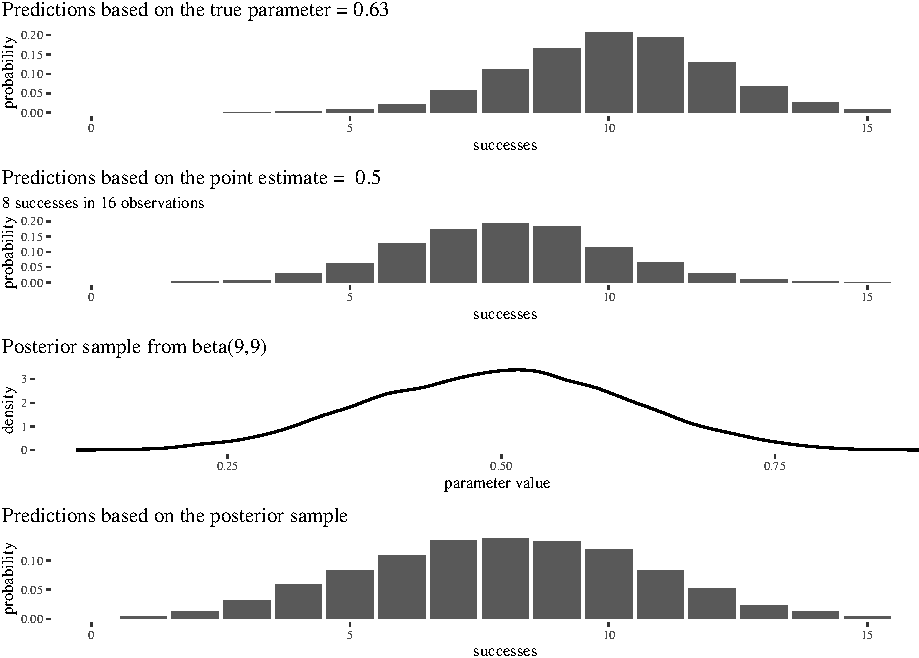
\includegraphics[width=0.8\linewidth]{paper-outline_files/figure-latex/fig:posteriorPrediction2-1} \end{center}


\caption{Real probability mass, probability mass calculated using a point estimate, sampling distribution from the posterior, and the posterior predictive distribution based on this sampling distribution.}
\label{fig:posteriorPrediction}
\end{figure}

The PMF based on a point estimate is further off from the real PMF than
the posterior predictive distribution. For instance, if we ask about the
probability of the outcome being at least 9 successes, the true answer
is 0.7984, the point estimate PMF tells us it is 0.4056, while the
posterior predictive distribution gives a somewhat better guess at
0.4277. A similar thing happens when we ask about the probability of the
outcome being at most 9 successes. The true answer is 0.3681, the
point-estimate-based answer is 0.778, while the posterior predictive
distribution yields 0.7051. More generally, we can use an
information-theoretic measure, Kullback-Leibler divergence, to quantify
how far the point-estimate PMF and the posterior predictive PMF are from
the true PMF.\^{}{[}A bit of explanation of this divergence measure.
Suppose we are dealing with a variable \(X\) with \(n\) distinct
possible discrete states \(x_1, \dots, x_n\) and consider two
probability mass functions \(p\) and \(q\) which express uncertainty
about the true value of \(X\) so that, say, on \(p\),
\(\pr(X=x_i)=p_i\). First, the uncertainty of a given distribution
\(p\), its \textbf{entropy}, is given by the sum of the logarithms of
surprise \(\nicefrac{1}{p_i}\) for all the possible values,
\(H(p) = \sum x_i \log \frac{1}{p_i} = - \sum p_i \log p_i\). Next,
suppose events arise according to \(p\), but we predict them using
\(q\). The \textbf{cross-entropy} is then\\
\$ \mathsf{H}(p, q) \& = \sum p\_i \log\_(q\_i)\$. This value is going
to be higher than the entropy of \(p\) if \(q\) is different from it.
Think of it as the uncertainty involved in using \(q\) to predict events
that arise according to \(p\).

Third, \textbf{Kullback-Leibler} divergence is the additional entropy
introduced by using \(q\) instead of \(p\) itself, that is, the
difference between cross-entropy and entropy: \begin{align*}
\mathsf{DKL}(p, q) & = H(p, q) - H(p)\\
&= - \sum p_i \log q_i   - \left(   - \sum p_i \log p_i \right) \\
& = - \sum p_i\left( \log q_i - \log p_i\right)\\
& =  \sum p_i\left( \log p_i - \log q_i\right)\\
& = \sum p_i \log \left( \frac{p_i}{q_i}\right)
\end{align*} \noindent  As it turns out, KL divergence is also the
expected difference in log probabilities. In particular, if \(p=q\) we
get \(DKL(p,p) = \sum p_i (\log_2 p_i - \log_2 p_i) = 0\), which works
out as it intuitively should be.{]}

In our particular case, the former distance is 0.7905638 and the latter
is 0.5681121.

This result can be generalized. We repeat the simulation 1000 times,
each time with a new true parameter, a new sample size, and a new
sample. Every time the three PMFs are constructed using the methods we
described. Figure \ref{fig:kldsPlots} displays the empirical
distribution of the results of such a simulation, where the differences
are measured by the Kullback-Leibler divergence. A positive difference
indicates that the distribution based on the point-estimate was further
from the true PMF than the posterior predictive distribution. Notably,
the mean difference is 0.865, the median difference is 0.044, and the
distribution is asymmetrical, as there are multiple cases of huge
differences favoring posterior predictive distributions over point-based
predictions. All in all, accuracy-wise, point-estimate-based PMFs are
systematically worse than the posterior predictive distribution.

\begin{figure}[H]

\begin{center}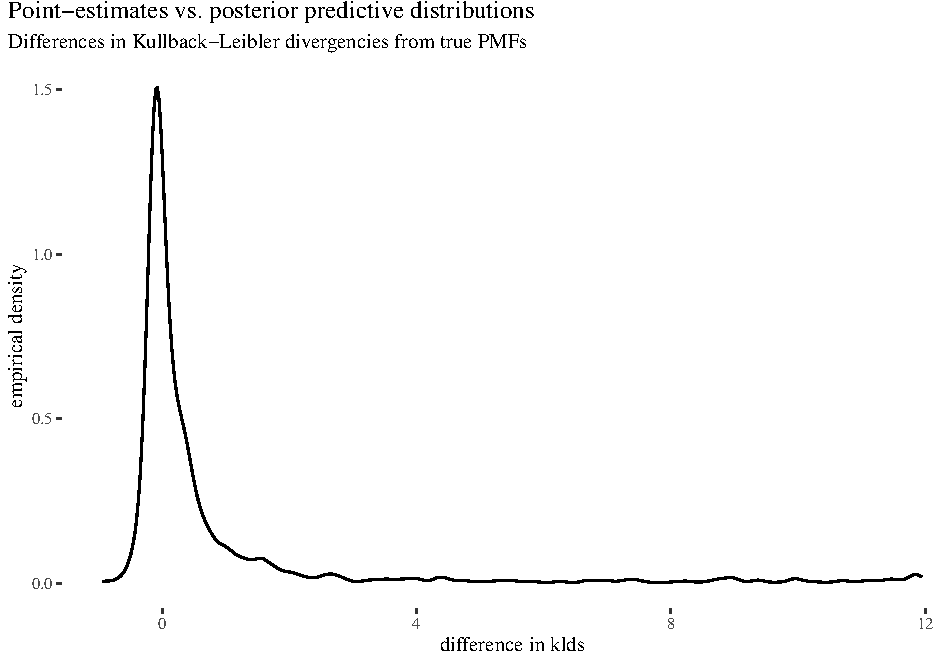
\includegraphics[width=0.7\linewidth]{paper-outline_files/figure-latex/fig:kldsPlots-1} \end{center}
\caption{Differences in Kullback-Leibler divergencies from the true distributions, comparing the distributions obtained using point estimates and posterior predictive distributions. Positive values indicate the point-estimate-based PMF was further from the true distribution than the posterior predictive distribution.}
\label{fig:kldsPlots}
\end{figure}

\hypertarget{conceptual-issues}{%
\subsection{Conceptual issues}\label{conceptual-issues}}

Accuracy considerations aside, we will now engage with the more
conceptual points. Taroni et al. (2015) argue that since first-order
probabilities capture your uncertainty about a proposition of interest,
second-order probabilities are supposed to capture your uncertainty
about how uncertain you are, and that ``estimating'' your first-order
uncertainties is unnecessary. They think that you can simply figure out
your fair odds in a suitable bet on the proposition in question, and the
fair odds track your unique, first-order uncertainty without any
uncertainty about it. But this point can be questioned. For one thing,
the betting interpretation of probability is not
uncontroversial.\footnote{See textbooks in formal epistemology (D.
  Bradley, 2015; Titelbaum, 2020).} In addition, even granting the
betting interpretation, it need not be implausible to say that we
sometimes are uncertain about what we think the fair bets are or what
our first-order uncertainties are.\footnote{On a related score, the
  introspective axioms in epistemic logic---that is, if an agent knows
  (or doesn't know) \(p\), they also know that they (don't) know
  \(p\)---are by no means uncontroversial. See, for example, Williamson
  2000 (chapter 5)'s argument against the KK principle of positive
  introspection.}

Think again about an expert who gathers information about the allelic
frequency \(f\) of DNA matches in an available database, and starts with
a defensible \s{beta} prior with parameters \(\alpha, \beta\). Say the
expert observes \(s\) matches in a database of size \(n\). So the
population relative frequency the experts is estimating should follow
the \(\s{beta}(\alpha + s + 1 ,\beta + n - s)\) distribution. So far,
nothing controversial happens---the expert is estimating the relevant
population frequency. Assuming the conditions are pristine (the expert
has no modeling uncertainty, rules out laboratory errors, and so on),
the beta distribution can be used to inform the expert's subjective
uncertainty. But uncertainty about what? The (estimated) population
frequency can serve to attach a probability to the proposition
\emph{a match is observed  if another person, unrelated to the suspect, is the source of the trace}.
Admittedly, if only this proposition is being considered, it is yet not
clear what second-order uncertainties would be uncertainties about. But
the expert also considers a continuum of propositions, each of the form
\emph{the true population frequency is $\theta$} for each
\(\theta\in [0,1]\). A density over \(\theta\) models the comparative
plausibility that the expert assigns to such propositions in light of
the evidence. So if one were worried that there were no propositions
that the expert could be ``second-order'' uncertain about, there
actually are plenty. In particular, if \(\theta\) is a population
frequency, gauging which density captures the extent to which the
evidence justifies various estimates of that frequency is the same as
gauging the comparative plausibility of the corresponding propositions
about the population frequencies.\footnote{Perhaps, this should no
  longer be called ``estimation'', but the the connection with
  estimation is strong enough to justify this terminology. In the end,
  this is a verbal discussion that we will not get into.}

More generally, evidence justifies first-order probability assignments
to various degrees. Suppose there is no evidence about the bias of a
coin. Then, each first-order uncertainty about it would be equally
(un)-justified. (If you like to think in terms of bets, the evidence
would give no reason to prefer any particular odds as fair.) If,
instead, we know the coin is fair, the evidence clearly selects one
preferred value, .5. (Again, if you like the betting metaphor, 1:1 would
be the preferred betting odds.) But often the evidence is stronger than
the former case and weaker than the latter case. Consider, for example,
propositions about population frequencies in light of the results of
observations. In such circumstances, the evidence justifies different
values of first-order uncertainty to various degrees, and densities
simply capture the extent to which different first-order uncertainties
are supported by the evidence.

We conclude this section by examining two additional points raised by
Taroni et al. (2015). The first---which we already alluded to
earlier---is that first-order probabilities are not ``states of nature''
and so cannot be estimated. It is unclear why only states of nature can
be estimated. Mathematicians use approximate methods to estimate answers
to fairly abstract questions ,not obviously related to ``states of
nature'', whatever these are. So, estimation should make sense whenever
there are some objective answers that we can approximate to a greater or
lesser extent.\footnote{Taroni et al. (2015) makes the same point for
  likelihood ratios. They argue that there is no ``meaningful state of
  nature equivalent for the likelihood ratio in its entirety, as it is
  given by a ratio of two conditional probabilities?'' But if it is
  meaningful to estimate two conditional probabilities (that is,
  frequencies in the population), or to compare the relative
  plausibility of various propositions about them in terms of density,
  it is equally meaningful to estimate any function of the numbers
  involved. Otherwise it would also be meaningless to try to estimate
  the body mass index (BMI) of an average 21 years old male student in
  the USA just because BMI is a ratio of other quantities.}

Second, Taroni et al. (2015) argue that once we allow second-order
probability, we run into the threat of infinite regress. But do we?
Surely, they would agree that one can be uncertain about a statistical
model. But this can be the case even if this model spits out a point
estimate rather than a density. If you think the possibility of putting
uncertainty on top of propositions about possible values of a
first-order parameter leaves us in an epistemically hopeless situation,
you might have hard time explaining why your point estimation is in a
better situation. After all, if asking further questions about
probabilities up the hierarchy is always justified, we can keep asking
about the probability of a point-estimate-spitting model, the
probability of that probability, and so on.

Perhaps the problem at issue is just one of complexity. Admittedly,
second-order estimation is more complex than relying on point estimates.
But we hope to have convinced the reader this complexity is worth the
effort. What about more complex models going third-order? If a workable
approach can accomplish that---and the additional complexity pays
off---we are all for going third-order. The fact that more complex
models can always be built hardly lead us into a vicious infinite
regress. Rather, it is an indication that our models of uncertainty
can---in principle---always be improved.

\hypertarget{references}{%
\section*{References}\label{references}}
\addcontentsline{toc}{section}{References}

\hypertarget{refs}{}
\begin{CSLReferences}{1}{0}
\leavevmode\vadjust pre{\hypertarget{ref-bradley2015critical}{}}%
Bradley, D. (2015). \emph{A critical introduction to formal
epistemology}. Bloomsbury Publishing.

\leavevmode\vadjust pre{\hypertarget{ref-bradley2012scientific}{}}%
Bradley, S. (2012). \emph{Scientific uncertainty and decision making}
(PhD thesis). London School of Economics; Political Science (University
of London).

\leavevmode\vadjust pre{\hypertarget{ref-bradley2019imprecise}{}}%
Bradley, S. (2019). {Imprecise Probabilities}. In E. N. Zalta (Ed.),
\emph{The {Stanford} encyclopedia of philosophy} ({S}pring 2019).
\url{https://plato.stanford.edu/archives/spr2019/entries/imprecise-probabilities/};
Metaphysics Research Lab, Stanford University.

\leavevmode\vadjust pre{\hypertarget{ref-CampbellMoore2020accuracy}{}}%
Campbell-Moore, C. (2020). \emph{Accuracy and imprecise probabilities}.

\leavevmode\vadjust pre{\hypertarget{ref-Carr2020impreciseEvidence}{}}%
Carr, J. R. (2020). Imprecise evidence without imprecise credences.
\emph{Philosophical Studies}, \emph{177}(9), 2735--2758.
\url{https://doi.org/10.1007/s11098-019-01336-7}

\leavevmode\vadjust pre{\hypertarget{ref-Dahlman2022Information}{}}%
Dahlman, C., \& Nordgaard, A. (2022). \emph{Information economics in the
criminal standard of proof}.

\leavevmode\vadjust pre{\hypertarget{ref-deadman1984fiber2}{}}%
Deadman, H. A. (1984a). Fiber evidence and the wayne williams trial
(conclusion). \emph{FBI L. Enforcement Bull.}, \emph{53}, 10--19.

\leavevmode\vadjust pre{\hypertarget{ref-deadman1984fiber1}{}}%
Deadman, H. A. (1984b). Fiber evidence and the wayne williams trial
(part i). \emph{FBI L. Enforcement Bull.}, \emph{53}, 12--20.

\leavevmode\vadjust pre{\hypertarget{ref-Dietrich2016pooling}{}}%
Dietrich, F., \& List, C. (2016). Probabilistic opinion pooling. In A.
Hajek \& C. Hitchcock (Eds.), \emph{Oxford handbook of philosophy and
probability}. Oxford: Oxford University Press.

\leavevmode\vadjust pre{\hypertarget{ref-Lee2017impreciseEpistemology}{}}%
Elkin, L. (2017). \emph{Imprecise probability in epistemology} (PhD
thesis). Ludwig-Maximilians-Universit{ä}t;
Ludwig-Maximilians-Universität München.

\leavevmode\vadjust pre{\hypertarget{ref-Elkin2018resolving}{}}%
Elkin, L., \& Wheeler, G. (2018). Resolving peer disagreements through
imprecise probabilities. \emph{Noûs}, \emph{52}(2), 260--278.
\url{https://doi.org/10.1111/nous.12143}

\leavevmode\vadjust pre{\hypertarget{ref-VanFraassen2006vague}{}}%
Fraassen, B. C. V. (2006). Vague expectation value loss.
\emph{Philosophical Studies}, \emph{127}(3), 483--491.
\url{https://doi.org/10.1007/s11098-004-7821-2}

\leavevmode\vadjust pre{\hypertarget{ref-Gardenfors1982unreliable}{}}%
Gärdenfors, P., \& Sahlin, N.-E. (1982). Unreliable probabilities, risk
taking, and decision making. \emph{Synthese}, \emph{53}(3), 361--386.
\url{https://doi.org/10.1007/bf00486156}

\leavevmode\vadjust pre{\hypertarget{ref-joyce2005probabilities}{}}%
Joyce, J. M. (2005). How probabilities reflect evidence.
\emph{Philosophical Perspectives}, \emph{19}(1), 153--178.

\leavevmode\vadjust pre{\hypertarget{ref-Kaplan1968decision}{}}%
Kaplan, J. (1968). Decision theory and the fact-finding process.
\emph{Stanford Law Review}, \emph{20}(6), 1065--1092.

\leavevmode\vadjust pre{\hypertarget{ref-keynes1921treatise}{}}%
Keynes, J. M. (1921). \emph{A treatise on probability, 1921}. London:
Macmillan.

\leavevmode\vadjust pre{\hypertarget{ref-konek2013foundations}{}}%
Konek, J. (2013). \emph{New foundations for imprecise bayesianism} (PhD
thesis). University of Michigan.

\leavevmode\vadjust pre{\hypertarget{ref-Kyburg1961}{}}%
Kyburg, H. E. (1961). \emph{Probability and the logic of rational
belief}. Wesleyan University Press.

\leavevmode\vadjust pre{\hypertarget{ref-kyburg2001uncertain}{}}%
Kyburg Jr, H. E., \& Teng, C. M. (2001). \emph{Uncertain inference}.
Cambridge University Press.

\leavevmode\vadjust pre{\hypertarget{ref-Levi1974ideterminate}{}}%
Levi, I. (1974). On indeterminate probabilities. \emph{The Journal of
Philosophy}, \emph{71}(13), 391. \url{https://doi.org/10.2307/2025161}

\leavevmode\vadjust pre{\hypertarget{ref-Levi1980enterprise}{}}%
Levi, I. (1980). \emph{The enterprise of knowledge: An essay on
knowledge, credal probability, and chance}. MIT Press.

\leavevmode\vadjust pre{\hypertarget{ref-Mayo-Wilson2016scoring}{}}%
Mayo-Wilson, C., \& Wheeler, G. (2016). Scoring imprecise credences: A
mildly immodest proposal. \emph{Philosophy and Phenomenological
Research}, \emph{92}(1), 55--78.
\url{https://doi.org/10.1111/phpr.12256}

\leavevmode\vadjust pre{\hypertarget{ref-Rinard2013against}{}}%
Rinard, S. (2013). Against radical credal imprecision. \emph{Thought: A
Journal of Philosophy}, \emph{2}(1), 157--165.
\url{https://doi.org/10.1002/tht3.84}

\leavevmode\vadjust pre{\hypertarget{ref-Schoenfield2017accuracy}{}}%
Schoenfield, M. (2017). The accuracy and rationality of imprecise
credences. \emph{Noûs}, \emph{51}(4), 667--685.
\url{https://doi.org/10.1111/nous.12105}

\leavevmode\vadjust pre{\hypertarget{ref-seidenfeld2012forecasting}{}}%
Seidenfeld, T., Schervish, M., \& Kadane, J. (2012). Forecasting with
imprecise probabilities. \emph{International Journal of Approximate
Reasoning}, \emph{53}, 1248--1261.
\url{https://doi.org/10.1016/j.ijar.2012.06.018}

\leavevmode\vadjust pre{\hypertarget{ref-Sjerps2015Uncertainty}{}}%
Sjerps, M. J., Alberink, I., Bolck, A., Stoel, R. D., Vergeer, P., \&
Zanten, J. H. van. (2015). {Uncertainty and LR: to integrate or not to
integrate, that's the question}. \emph{Law, Probability and Risk},
\emph{15}(1), 23--29. \url{https://doi.org/10.1093/lpr/mgv005}

\leavevmode\vadjust pre{\hypertarget{ref-Stewart2018pooling}{}}%
Stewart, R. T., \& Quintana, I. O. (2018). Learning and pooling, pooling
and learning. \emph{Erkenntnis}, \emph{83}(3), 1--21.
\url{https://doi.org/10.1007/s10670-017-9894-2}

\leavevmode\vadjust pre{\hypertarget{ref-Sturgeon2008grain}{}}%
Sturgeon, S. (2008). Reason and the grain of belief. \emph{No{û}s},
\emph{42}(1), 139--165. Retrieved from
\url{http://www.jstor.org/stable/25177157}

\leavevmode\vadjust pre{\hypertarget{ref-Taroni2015Dismissal}{}}%
Taroni, F., Bozza, S., Biedermann, A., \& Aitken, C. (2015). {Dismissal
of the illusion of uncertainty in the assessment of a likelihood ratio}.
\emph{Law, Probability and Risk}, \emph{15}(1), 1--16.
\url{https://doi.org/10.1093/lpr/mgv008}

\leavevmode\vadjust pre{\hypertarget{ref-Titelbaum2020Fundamentals-of}{}}%
Titelbaum, M. G. (2020). \emph{Fundamentals of bayesian epistemology}.

\leavevmode\vadjust pre{\hypertarget{ref-walley1991statistical}{}}%
Walley, P. (1991). \emph{Statistical reasoning with imprecise
probabilities}. Chapman; Hall London.

\end{CSLReferences}

\end{document}
